%%%%%%%%%%%%%%%%%%%%%%%%%%%%%%%%%%%%%%%%%
% Professional Newsletter Template
% LaTeX Template
% Version 1.0 (09/03/14)
%
% Created by:
% Bob Kerstetter (https://www.tug.org/texshowcase/) and extensively modified by:
% Vel (vel@latextemplates.com)
% 
% This template has been downloaded from:
% http://www.LaTeXTemplates.com
%
% License:
% CC BY-NC-SA 3.0 (http://creativecommons.org/licenses/by-nc-sa/3.0/)
%
%%%%%%%%%%%%%%%%%%%%%%%%%%%%%%%%%%%%%%%%%

\documentclass[9pt]{extarticle} % The default font size is 10pt; 11pt and 12pt are alternatives

%%%%%%%%%%%%%%%%%%%%%%%%%%%%%%%%%%%%%%%%%
% Professional Newsletter Template
% Structural Definitions File
% Version 1.0 (09/03/14)
%
% Created by:
% Vel (vel@latextemplates.com)
% 
% This file has been downloaded from:
% http://www.LaTeXTemplates.com
%
% License:
% CC BY-NC-SA 3.0 (http://creativecommons.org/licenses/by-nc-sa/3.0/)
%
%%%%%%%%%%%%%%%%%%%%%%%%%%%%%%%%%%%%%%%%%

%----------------------------------------------------------------------------------------
%	REQUIRED PACKAGES
%----------------------------------------------------------------------------------------

\usepackage{listings}
\usepackage{graphicx} % Required for including images
\usepackage{microtype} % Improved typography
\usepackage{multicol} % Used for the two-column layout of the document
\usepackage{booktabs} % Required for nice horizontal rules in tables
\usepackage{wrapfig} % Required for in-line images
\usepackage{float} % Required for forcing figures not to float with the [H] parameter
\usepackage[utf8]{inputenc}
\usepackage{fancyhdr}

%------------------------------------------------
% Fonts

\usepackage{charter} % Use the Charter font as the main document font
\usepackage{courier} % Use the Courier font for \texttt (monospaced) only
\usepackage[T1]{fontenc} % Use T1 font encoding

%------------------------------------------------
% List Separation

\usepackage{enumitem} % Required to customize the list environments
\setlist{noitemsep,nolistsep} % Remove spacing before, after and within lists for a compact look

%------------------------------------------------
% Figure and Table Caption Styles

\usepackage{caption} % Required for changing caption styles
\captionsetup[table]{labelfont={bf,sf},labelsep=period,justification=justified} % Specify the table caption style
\captionsetup[figure]{labelfont={sf,bf},labelsep=period,justification=justified, font=small} % Specify the figure caption style
\setlength{\abovecaptionskip}{10pt} % Whitespace above captions

%------------------------------------------------
% Spacing Between Paragraphs

\makeatletter
\usepackage{parskip}
\setlength{\parskip}{6pt}
\newcommand{\@minipagerestore}{\setlength{\parskip}{6pt}}
\makeatother

%----------------------------------------------------------------------------------------
%	PAGE MARGINS AND SPACINGS
%----------------------------------------------------------------------------------------

\textwidth = 7 in % Text width
\textheight = 10 in % Text height
\oddsidemargin = -18pt % Left side margin on odd pages
\evensidemargin = -18pt % Left side margin on even pages
\topmargin = -36pt % Top margin
\headheight = 0pt % Remove the header by setting its space to 0
\headsep = 0pt % Remove the space between the header and top of the page
\parskip = 2pt % Space between paragraph
\parindent = 0.0in % Paragraph indentation
\pagestyle{empty} % Disable page numbering

%----------------------------------------------------------------------------------------
%	COLORS
%----------------------------------------------------------------------------------------

\usepackage[dvipsnames,svgnames]{xcolor} % Required to specify custom colors

\definecolor{altncolor}{rgb}{.8,0,0} % Dark red
%\definecolor{altncolor}{rgb}{.2,.4,.8} % Dark blue
%\definecolor{altncolor}{rgb}{.84,.16,.16} % Red

\usepackage[colorlinks=true, linkcolor=altncolor, anchorcolor=altncolor, citecolor=altncolor, filecolor=altncolor, menucolor=altncolor, urlcolor=altncolor]{hyperref} % Use the color defined above for all links

%----------------------------------------------------------------------------------------
%	BOX STYLES
%----------------------------------------------------------------------------------------

\usepackage[framemethod=TikZ]{mdframed}% Required for creating boxes
\mdfdefinestyle{sidebar}{
    linecolor=black, % Outer line color
    outerlinewidth=0.5pt, % Outer line width
    roundcorner=0pt, % Amount of corner rounding
    innertopmargin=10pt, % Top margin
    innerbottommargin=10pt, % Bottom margin
    innerrightmargin=10pt, % Right margin
    innerleftmargin=10pt, % Left margin
    backgroundcolor=white, % Box background color
    frametitlebackgroundcolor=white, % Title background color
    frametitlerule=false, % Title rule - true or false
    frametitlerulecolor=white, % Title rule color
    frametitlerulewidth=0.5pt, % Title rule width
    frametitlefont=\Large, % Title heading font specification
    font=\small
}

\mdfdefinestyle{intextbox}{
    linecolor=black, % Outer line color
    outerlinewidth=0.5pt, % Outer line width
    roundcorner=10pt, % Amount of corner rounding
    innertopmargin=7pt, % Top margin
    innerbottommargin=7pt, % Bottom margin
    innerrightmargin=7pt, % Right margin
    innerleftmargin=7pt, % Left margin
    backgroundcolor=white, % Box background color
    frametitlebackgroundcolor=white, % Title background color
    frametitlerule=false, % Title rule - true or false
    frametitlerulecolor=white, % Title rule color
    frametitlerulewidth=0.5pt, % Title rule width
    frametitlefont=\Large % Title heading font specification
}

%----------------------------------------------------------------------------------------
%	HEADING STYLE
%----------------------------------------------------------------------------------------

\newcommand{\heading}[2]{ % Define the \heading command
\vspace{#2} % White space above the heading
{\begin{center}\Large\textbf{#1}\end{center}} % The heading style
\vspace{#2} % White space below the heading
}

\newcommand{\BackToContents}{\hyperlink{contents}{{\small Back to Contents}}} % Define a command for linking back to the contents of the newsletter % Include the document which specifies all packages and structural customizations for this template

\begin{document}

%--------------------------------------------------------------------------------
% HEADER DETAILS
%--------------------------------------------------------------------------------

\pagestyle{fancy}
\fancyhf{}
\chead{segfault@csh.rit.edu}
\rhead{\today}
\lhead{Volume XLVIII Issue \#3}
\addtolength\footskip{-15px}
\cfoot{"Wait you need water to make coffee!?!" - Ben Grawi (bgrawi)}
\setlength{\headsep}{0.1in}

%----------------------------------------------------------------------------------------
%	HEADER IMAGE
%----------------------------------------------------------------------------------------

\begin{figure}[H]
\centering\vspace{0.5cm}
\includegraphics[width=0.8\linewidth]{imgs/segfault.png}
\end{figure}

%--------------------------------------------------------------------------------
% HEADER QUOTE
%--------------------------------------------------------------------------------

\vspace{-15px}
\begin{quote}
\centering
\textbf{\textit{Yes I do mine your data}}
\end{quote}
\vspace{10px}

%----------------------------------------------------------------------------------------
%	SIDEBAR - FIRST PAGE
%----------------------------------------------------------------------------------------

\vspace{-0.5cm}\begin{minipage}[t]{.35\linewidth} % Mini page taking up 35% of the actual page
\begin{mdframed}[style=sidebar,frametitle={}] % Sidebar box

%-----------------------------------------------------------

\hypertarget{contents}{\textbf{{\large This week on floor\ldots}}} % \hypertarget provides a label to reference using \hyperlink{label}{link text}
\begin{itemize}
\item \hyperlink{firstnews}{Jaccard Distance Metric}
\item \hyperlink{secondnews}{NNTP Data Mining}
\end{itemize}

\centerline {\rule{.75\linewidth}{.25pt}} % Horizontal line

%-----------------------------------------------------------

\textbf{Notable Upcoming Events:}
\begin{enumerate}[leftmargin=0.2cm]
\item \textbf{<EVENT NAME>} <DATE + TIME> \\
	<DESCRIPTION>
\\
\item \textbf{<EVENT NAME>} <DATE + TIME> \\
	<DESCRIPTION>
\\
\end{enumerate}

%-----------------------------------------------------------


\textbf{<TITLE>} \\
<SHORT SECTION>
\\

%-----------------------------------------------------------

\captionof*{table}{Voting Results}
\begin{tabular}{lcr}

Vote & Cost & Result \\
\midrule
<NAME> & \$<MONEY> & <STATUS> \\
\bottomrule
\end{tabular}

%-----------------------------------------------------------

\end{mdframed}
\end{minipage}\hfill % End the sidebar mini page 
%
%----------------------------------------------------------------------------------------
%	MAIN BODY - FIRST PAGE
%----------------------------------------------------------------------------------------
%
\begin{minipage}[t]{.61\linewidth} % Mini page taking up 61% of the actual page
\vspace{-0.4cm}
\hypertarget{firstnews}{\heading{Jaccard Distance Metric}{6pt}}

The Jaccard index, also known as the Jaccard similarity coefficient (originally coined coefficient de communauté by Paul Jaccard), is a statistic used for comparing the similarity and diversity of sample sets. The Jaccard coefficient measures similarity between finite sample sets, and is defined as the size of the intersection divided by the size of the union of the sample sets: \\
\\
\begingroup
    \fontsize{18pt}{12pt}\selectfont
	\centerline{d(x, y) = $\frac{\vert\ x\ \cap\ y\ \vert}{\vert\ x\ \cup\ y\ \vert}$}
\endgroup
\\

An important class of problems that Jaccard addresses well is that of finding textually similar documents in a large corpus such as the Web or a collection of news articles. Many of these involve finding duplicates or near duplicated. First, let us observe that testing whether two documents are exact duplicates is easy; just compare the two documents character-by-character. However, in many applications, the documents are not identical, yet they share large portions of their text. Here are some examples: \\
\\
\textbf{Plagiarism:} \\
Finding plagiarized documents tests our ability to find textual similarity. The plagiarizer may extract only some parts of a document for his own. He may alter a few words and may alter the order in which the sentences appear. No simple process of comparing documents character-by-character will detect sophisticated plagiarism. \\
\\
\textbf{Mirror Page:} \\
It is common for important or popular web sites to be duplicated at a number of hosts, in order to share the load. The pages of these \textit{mirror} sites will be quite similar, but are rarely identical. For instance, they might each contain information associated with their particular host, and they might contain links to the other mirror sites but not to themselves. It is important to be able to detect similar pages of these kinds, because search engines produce better results if they avoid showing two pages that are nearly identical within the first page of results. \\
\\
\textbf{Articles from the Same Source:} \\
It is common for one reporter to write a news article that gets distributed say through the Associated Press, to many newspapers, which then publish the article on their sites. Each newspaper changes the article somewhat. They may cut out paragraphs, or even add material of their own. they most likely will surround the article with their own logo or adds. News aggregators try to find all versions of such an article, in order to show only one, and that task requires finding when two web pages are textually similar, although not identical.  

%-----------------------------------------------------------


\end{minipage} % End the main body - first page mini page

\pagebreak

\hypertarget{secondnews}{\heading{NNTP Data Mining}{6pt}} 

Some people wanted me to post the results of my data mining project of our NNTP server, so here is the abstract.  \\
\\
Our server has over 125,000 posts but I only used the last 3 years of data, which was 8,145 posts. Data mining was done using agglomerative clustering over the body of the posts. Text-mining can be difficult to deal with since it cannot be represented in Euclidean space. To get around this, Jaccard similarity coefficient was used as the distance metric since it is able to effectively find similar data. It produces a   value between one and zero where zero means the two items are identical and one means they have nothing in common. Preprocessing was done on the data to remove stop words, normalize the data, and to preform dimensionality reduction. \\
\\
\centerline{\textbf{Results}}

\begin{multicols}{2}

\centerline{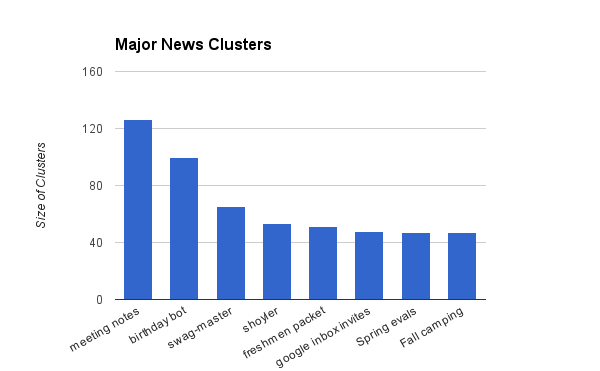
\includegraphics[width=\linewidth]{imgs/2016-02-15-clusters.png}}

As shown here, the biggest cluster was a combination of all the meeting notes posted by our glorious e-board members. This cluster was easy to find since most of our e-board members post notes following a very similar format and talk about similar material. An interesting side note is that \textbf{Marck} Billow generated a cluster of his own due to how unique his meeting notes are. He just had to be special...

\centerline{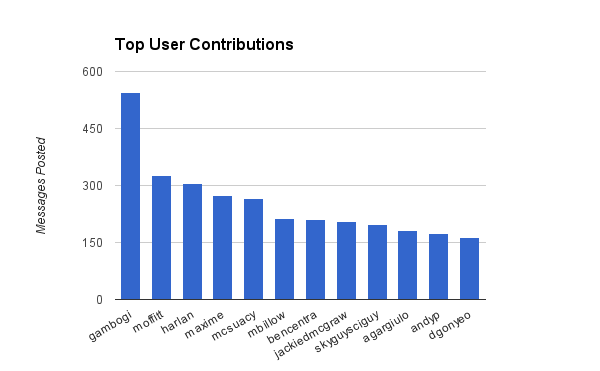
\includegraphics[width=\linewidth]{imgs/2016-02-15-users.png}}

Here are the most active users of our NNTP server. As shown here, our top 12 users accounted for 37.58\% of the total posts in the last 3 years. \\
\\


\vfill
\columnbreak

\centerline{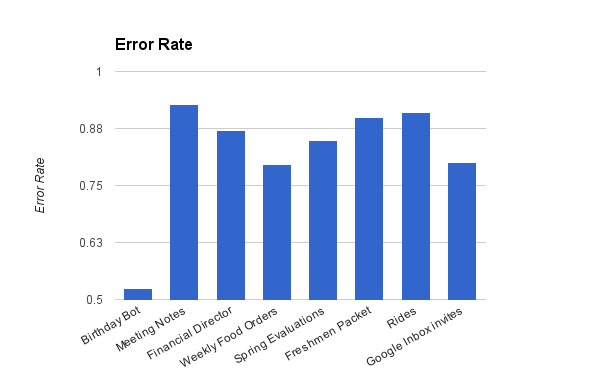
\includegraphics[width=\linewidth]{imgs/2016-02-15-error.png}}

The error rate of a cluster was generated by the average distance between every post in the cluster. This forms a value between 1 and 0, in which 0 means all posts are identical and 1 means that there are no shared similarities. The results from this graph make sense since the birthday bot posts very similarly formatted messages so that cluster has the lowest differences between posts. Weekly food orders tend to involve the same people and all be about the same topic so that cluster also has a low error rate. 



Let me know if you have additional questions about my findings. 

\end{multicols}

\end{document} 